% !TeX encoding=utf8
% !TeX spellcheck = de_CH_frami

\chapter{Einleitung}
\label{sec:einleitung}
%Im Rahmen der Bachelorarbeit werden Buchungsdaten von Interhome analysiert, um daraus Erkenntnisse zu gewinnen. In der Einleitung wird die Aufgabenstellung erläutert, sowie Abgrenzungen definiert.
 
 

%\section{Aufgabenstellung}
%\label{sec:vorgehen:aufgabenstellung}
%Nachfolgend ist die Aufgabenstellung aufgeführt, wie sie für die Projektfreigabe eingereicht wurde.

\section{Ausgangslage}
\label{sec:einleitung:ausgangslage}

Die Interhome AG ist eine Internationale Firma mit Büros in 10 Ländern. Sie vertreibt Ferienhäuser und -wohnungen (Objekte) auf einer Webseite welche in 26 Domains und 14 Sprachen aufgerufen werden kann. Darauf können Kunden Objekte suchen und Buchen. Dazu muss der User eine Destination auswählen und kann daraufhin verschiedenen Objekte ansehen. Diese haben einen Namen, Bilder und diverse Attribute. Beispiele solcher Attribute sind, ob die Wohnung einen Fernseher besitzt, Tiere erlaubt sind oder eine Sauna vorhanden ist.

Die Buchungen werden in das \gls{irent} gespeichert. Die gesammelten Daten werden von einem Recommender System, welches von Interhome entwickelt wurde, analysiert. Weitere Untersuchungen der Daten finden im Moment nicht statt.

\section{Organisationsstruktur}
\label{sec:einleitung:ausgangslage:organisationsstruktur}
Die Hotelplan Holding AG ist eine Tochtergesellschaft des Migros-Genossenschafts-Bundes. Darin sind verschiedene \glspl{sbu} angesiedelt, unter anderem auch die Interhome AG. Veranschaulicht wird das in \cref{fig:einleitung:organisationsstruktur:1}.
\label{sec:einleitung:organisationsstruktur}
\begin{figure}[h]
	\RawFloats
	\centering
	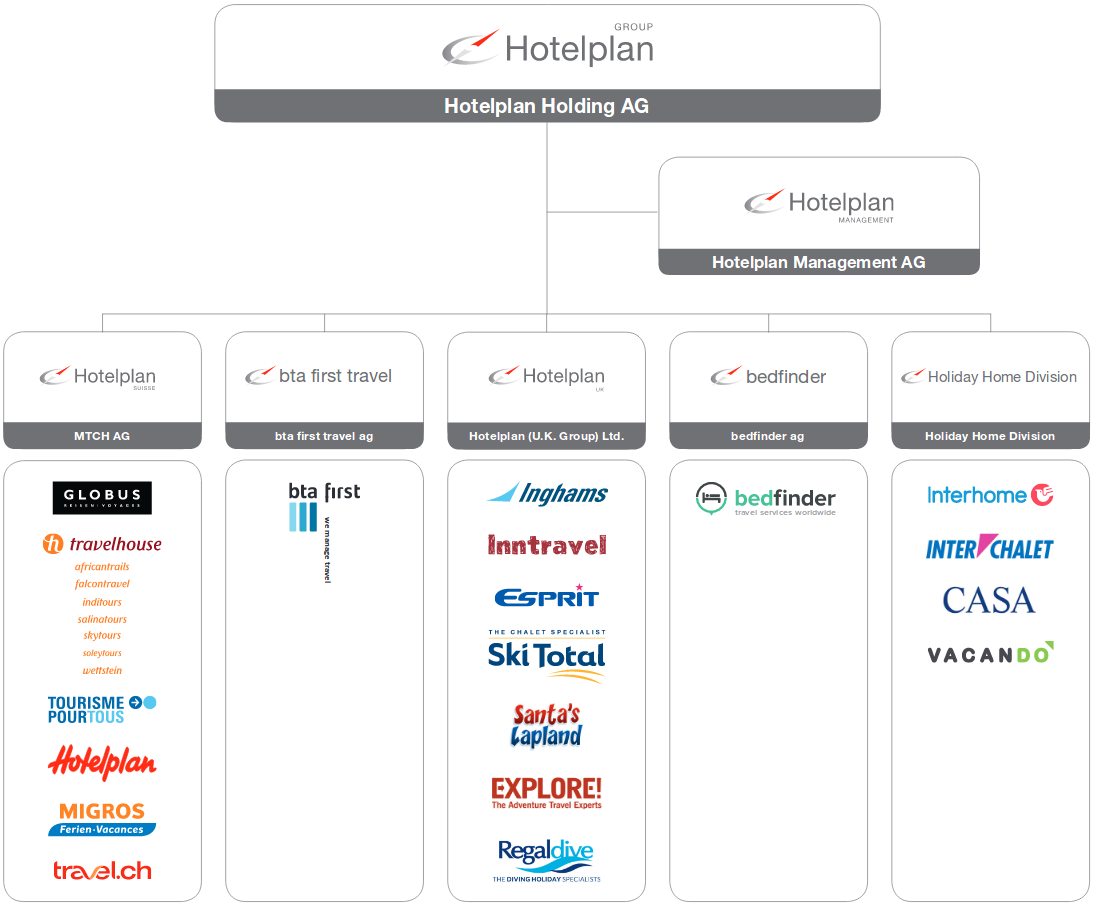
\includegraphics[width=0.7\textwidth]{images/organisationsstruktur}
	\caption{Organisationsstruktur der Hotelplan Group}
	\label{fig:einleitung:organisationsstruktur:1}
\end{figure}

In der \cref{fig:einleitung:organisationsstruktur:2} werden die Marken der verschiedenen \glspl{sbu} aufgeführt.
\begin{table}[h] 
	\caption{Markenaufstellung der Hotelplan Management AG}
	\centering
	\rowcolors{1}{tablebodycolor}{tablerowcolor}
	\label{fig:einleitung:organisationsstruktur:2}
	\begin{tabular}{ | c | c | c |} 
		\hline 		
		\rowcolor{tableheadcolor}
		\bfseries \gls{sbu} & \bfseries Marke & \bfseries Portal \\ \hline 
		Hotelplan Managment AG & Hotelplan Management & \href{http://www.hotelplan.com}{www.hotelplan.com} \\ \hline 
		MTCH AG & Globus Reisen & \href{http://www.globusreisen.ch}{www.globusreisen.ch} \\ \hline 
		MTCH AG & Travelhouse & \href{http://www.travelhouse.ch}{www.travelhouse.ch} \\ \hline 
		MTCH AG & Tourisme pour Tous & \href{http://www.tourismepourtous.ch/}{www.tourismepourtous.ch} \\ \hline 
		MTCH AG & Hotelplan & \href{http://www.hotelplan.ch}{www.hotelplan.ch} \\ \hline 
		MTCH AG & Migros Ferien & \href{http://www.migros-ferien.ch}{www.migros-ferien.ch} \\ \hline 
		MTCH AG & Travelwindow & \href{http://www.travel.ch}{www.travel.ch} \\ \hline 
		bta first travel ag & bta first & \href{http://www.btafirst.com}{www.btafirst.com} \\ \hline 
		Hotelplan UK & Inghams & \href{http://www.inghams.co.uk}{www.inghams.co.uk} \\ \hline 
		Hotelplan UK & Inntravel & \href{http://www.inntravel.co.uk}{www.inntravel.co.uk} \\ \hline 
		Hotelplan UK & Esprit & \href{http://www.esprit-holidays.co.uk}{www.esprit-holidays.co.uk} \\ \hline 
		Hotelplan UK & Ski Total & \href{http://www.skitotal.com}{www.skitotal.com} \\ \hline 
		Hotelplan UK & Santa's Lapland & \href{http://www.santaslapland.com}{www.santaslapland.com} \\ \hline 
		Hotelplan UK & Explore & \href{http://www.explore.co.uk}{www.explore.co.uk} \\ \hline 
		Hotelplan UK & Regaldive & \href{http://www.regal-diving.co.uk}{www.regal-diving.co.uk} \\ \hline 
		bedfinder ag & Bedfinder & \href{http://www.bedfinder.com}{www.bedfinder.com} \\ \hline 
		Holiday Home Division & Interhome & \href{http://www.interhome.ch}{www.interhome.ch} \\ \hline 
		Holiday Home Division & Interchalet & \href{http://www.interchalet.de}{www.interchalet.de} \\ \hline 
		Holiday Home Division & Casa & \href{http://casa.interchalet.de}{casa.interchalet.de} \\ \hline 
		Holiday Home Division & Vacando & \href{http://www.vacando.ch}{www.vacando.ch} \\ \hline 
	\end{tabular}
\end{table}

\section{Ziel der Arbeit}
\label{sec:einleitung:ziel}
Das Ziel der Arbeit ist es, Interhome bei Entscheidungen zum Thema Marketing oder Einkauf zu unterstützen. Bislang hat man sich auf das Bauchgefühl verlassen. Durch eine Analyse von Buchungsdaten sollte den Entscheidungen von Interhome eine Grundlage gegeben werden. 

Der Einkauf sollte in Erfahrung bringen können, was zum Beispiel von den Kunden in der Schweiz am meisten gebucht wird. Sie sollen eine Anfrage dazu stellen können in der Form von: "Was für Objekte werden von Schweizern am meisten gebucht?". Das Resultat könnte sein: "Objekte, in Italien und maximal 500 Meter vom Meer entfernt sind". Dadurch weiss der Einkauf, dass eventuell mehr Objekte in Italien eingekauft werden müssen, welche weniger als 500 Meter vom Meer entfernt sind.

Das Marketing hingegen könnte eine solche Anfrage an die Analyse stellen: „Was für Objekte werden im Winter am meisten in Zermatt gebucht?“. Eine mögliche Antwort wäre: „Objekte welche unter CHF500 kosten und maximal 200 Meter von einem Skilift entfernt sind“. Solche Informationen können helfen, gezielter Werbung zu schalten. Auf der Webseite kann damit einem Benutzer, welcher eine Ferienwohnung in Zermatt im Winter sucht gezielter Objekte angezeigt werden. Nämlich solche, welche maximal CHF500 kosten und 200 Meter vom Skilift entfernt sind.

Um solche Fragen zu beantworten werden die Buchungsdaten von Interhome (Objekt, Zeitraum, Passagiere, etc.) verwendet und mit weiteren Daten (Geolocation, Wetterinformation) angereichert. 
Auf dem Endprodukt soll ein Mitarbeiter von Interhome in der Lage sein, eine Abfrage zu generieren, welche aus einem oder mehreren Attributen besteht. Die Applikation analysiert daraufhin die Daten mit Techniken des Data Mining, um eine Liste von Attributen zurück zu liefern, welche für die in der Abfrage aufgeführten Attributen am meisten Buchungen generieren. Die Elemente in der Antwort sollten gewichtet sein um das Resultat besser zu interpretieren.

\subsection{Beispiel}
Um dies besser zu veranschaulichen sollte hier ein Beispiel gemacht werden. Dazu ist in der \cref{fig:einleitung:ziel:1} eine Datenmenge aufgeführt. Aufgeteilt sind die Spalten in Objekt- und Kundendaten. Dies hat keinen weiteren Einfluss auf diese Arbeit und sollte lediglich zum besseren Verständnis führen. Die ersten 9 Spalten sind Rohdaten und das Wetter (letzte Spalte) muss zusätzlich angereichert werden.

\begin{table}[H] 
	\caption{Beispielhafte angereicherte Buchungsdaten}
	\centering
	\rowcolors{1}{tablebodycolor}{tablerowcolor}
	\label{fig:einleitung:ziel:1}
	\begin{tabular}{ | c | c | c | c | c | c | c | c | c | c |} 
		\hline 
		\rowcolor{tableheadcolor}
		\multicolumn{8}{|c|}{\bfseries Objektdaten} & \multicolumn{2}{c|}{\bfseries Kundendaten} \\ \hline
		
		\rowcolor{tableheadcolor}
		\bfseries \rotatebox{90}{ID} & \bfseries \rotatebox{90}{Objekt Ortschaft} & \bfseries \rotatebox{90}{Preis (CHF)} & \bfseries \rotatebox{90}{Tiere erlaubt} & \bfseries \rotatebox{90}{Grill vorhanden} & \bfseries \rotatebox{90}{Balkon vorhanden} & \bfseries \rotatebox{90}{Distanz zum Meer (m)} & \bfseries \rotatebox{90}{Distanz zum Skilift (m)} &  
		
		\bfseries \rotatebox{90}{Kunde Ortschaft} & \bfseries \rotatebox{90}{Wetter} \\ \hline 
		
1 & Saint-Tropez & 230 	& \checkmark & 			  &			   & 150	&		& Bern 		  & Sonne 	\\ \hline 
2 & Zermatt		 & 450 	& 			 & \checkmark & \checkmark & 		& 700	& Grindelwald & Schnee  \\ \hline 
3 & Saint-Tropez & 2301	& \checkmark & \checkmark & 		   & 190	& 		& Mallorca	  & Regen 	\\ \hline 
4 & Saint-Tropez & 879 	& \checkmark & 			  & \checkmark & 150	& 	 	& Nizza 	  & Regen 	\\ \hline 
5 & Saint-Tropez & 149 	& \checkmark & 			  & \checkmark & 350	& 	 	& Zürich	  & 		\\ \hline
6 & Berlin 		 & 873 	& 			 & \checkmark & 		   & 	 	&		& Nizza 	  & Regen	\\ \hline 
7 & Saint-Tropez & 620 	& \checkmark & \checkmark &  		   & 280 	&  		& Amsterdam	  & Regen	\\ \hline
\multicolumn{10}{|c|}{... mehr ...} \\ \hline 
	\end{tabular}
\end{table}

Als Beispiel möchte das Marketing wissen, was gebucht wird wenn es regnet. Die Anfrage lautet "`Wetter = Regen"' was auf die Elemente mit den IDs 3, 4, 6 und 7 zutrifft. Das Resultat der Abfrage ist in \cref{fig:einleitung:ziel:2} aufgeführt. Dort sind nur noch Elemente vorhanden, welche im Attribut "`Wetter"' den Wert "`Regen"' besitzen.

\begin{table}[H] 
	\caption{Resultat einer Anfrage}
	\centering
	\rowcolors{1}{tablebodycolor}{tablerowcolor}
	\label{fig:einleitung:ziel:2}
	\begin{tabular}{ | c | c | c | c | c | c | c | c | c | c |} 
		\hline 
		\rowcolor{tableheadcolor}
		\multicolumn{8}{|c|}{\bfseries Objektdaten} & \multicolumn{2}{c|}{\bfseries Kundendaten} \\ \hline
		
		\rowcolor{tableheadcolor}
		\bfseries \rotatebox{90}{ID} & \bfseries \rotatebox{90}{Objekt Ortschaft} & \bfseries \rotatebox{90}{Preis (CHF)} & \bfseries \rotatebox{90}{Tiere erlaubt} & \bfseries \rotatebox{90}{Grill vorhanden} & \bfseries \rotatebox{90}{Balkon vorhanden} & \bfseries \rotatebox{90}{Distanz zum Meer (m)} & \bfseries \rotatebox{90}{Distanz zum Skilift (m)} &  
		
		\bfseries \rotatebox{90}{Kunde Ortschaft} & \bfseries \rotatebox{90}{Wetter} \\ \hline 

3	& Saint-Tropez	& 2301 & \checkmark & \checkmark &				& 190	& 		& Mallorca	& Regen \\ \hline
4	& Saint-Tropez	& 1879 & \checkmark &			 & \checkmark	& 150	& 	 	& Nizza 	& Regen \\ \hline 
6	& Berlin 		& 873  &			& \checkmark & 				&		&		& Zürich 	& Regen	\\ \hline 
7	& Saint-Tropez	& 320  & \checkmark & \checkmark &  			& 180	&  		& Amsterdam	& Regen	\\ \hline
28  & Mallorca 		& 870  & 			& 			 & 				& 80	&		& Bern		& Regen \\ \hline
58  & Cannes 		& 1870 & \checkmark	& 			 & \checkmark	& 185	&		& Luzern	& Regen \\ \hline
99  & Saint-Tropez	& 1050 & \checkmark	& \checkmark & 				& 95	&		& Zürich	& Regen \\ \hline
	\end{tabular}
\end{table}

Diese Daten können nun Analysiert werden. Dabei werden jene Attribute gesucht, welche am häufigsten vorkommen. 
Das Resultat der Datenanalyse ist in diesem Fall "`Objekt Ortschaft = Saint-Tropez, Distanz zum Meer < 200 in 4/7 Buchungen"' (Buchungen mit den IDs 3, 4, 7, 99). Oder in Worten: "`In 57\% der selektieren Buchungen wurden Objekte in Saint-Tropez gebucht, welche maximal 200 Meter vom Meer entfernt sind."'. Sprich wenn es regnet, buchen viele Kunden in Saint-Tropez ein Objekt welches nahe am Meer liegt.

\subsection{Hypothesen}
Leider gibt es nur sehr grundlegendes Wissen über bestehende Muster der Buchungen von Interhome. Bekannt ist welche Destinationen oft gebucht wird. Die Häufigkeit von Attributekombinationen ist jedoch nicht erforscht. Nichts desto trotz werden hier einige Hypothesen darüber aufgestellt, was von den Algorithmen in dieser Arbeit für Daten gefunden werden sollen. Erfasst wurden diese Hypothesen in Zusammenarbeit mit der Interhome.

\paragraph{Hypothese 1} Die meisten Kunden von Interhome kommen aus der Schweiz oder Frankreich
\paragraph{Hypothese 2} Die meisten Buchungen werden für die Schweiz und für Frankreich getätigt.
\paragraph{Hypothese 3} Schweizer Kunden buchen meistens Objekte in der Schweiz.
\paragraph{Hypothese 4} Bei Destinationen mit Meer Anschluss werden öfters Objekte mit mehreren Schlafzimmern gebucht, da Familien eher Strandurlaub betreiben als Städtereisen.
\paragraph{Hypothese 5} In Schweizer Skiregionen werden die meisten Objekte gebucht weil die Gäste Skifahren gehen. Dazu müssen sie direkt am Skigebiet wohnen oder einen Anschluss dazu haben. Deshalb sollte diese Arbeit zeigen können, dass Objekte welche in Schweizer Skiregionen gebucht werden entweder nahe am Skilift liegen oder nahe am öffentlichen Verkehr.

%No filters:
%	Customer Country=ch						23338 - 20.94
%	Customer Country=fr						20709 - 18.58
%	Customer Country=de						16083 - 14.43
%	Customer Country=pl						12203 - 10.95
%	Customer Place=warszawa					2004 - 1.80
%	Customer Place=moscow					1311 - 1.18
%	Customer Place=paris					1136 - 1.02
%
%	Object Country=switzerland				22203 - 19.92
%	Object Country=france					15570 - 13.97
%	Object Region=valais					10056 - 9.02
%	Object Region=cote d'azur				3939 - 3.53
%	Object Region=savoie - haute savoie		3693 - 3.31
%	Object Region=costa blanca				3624 - 3.25
%	Object Place=norddeich					2989 - 2.68
%	Object Place=nendaz						2909 - 2.61
%	Object Place=zermatt					1532 - 1.37
%	Object Place=crans-montana				1479 - 1.33
%	Object Place=grindelwald				1442 - 1.29
%	Object Place=ascona						1215 - 1.09
%
%Customer, distances and location
%	IT: Weekly price=1 			953 - 50.48 
%		Close to pubt=1 		722 - 38.24 
%		Close to water=1 		472 - 25.00
%	FR: Weekly price=1 			9625 - 46.48
%		Close to water=1		6976 - 33.69
%		Object Country=france	6669 - 32.20
%		Close to sea=1 			6575 - 31.75
%	CH: Object Country=switzerland	11492 - 49.24
%		Close to pubt=1				9709 - 41.60
%		Weekly price=2				7274 - 31.17
%		Close to center=1			6015 - 25.77
%		
%Customer, location
%	CH: Object Country=switzerland	11492 - 49.24
%		Object Country=france		1714 - 7.34
%		Object Country=italy		1632 - 6.99
%		Object Country=spain		1212 - 5.19
%	CH:	Object Region=valais		4999 - 21.42
%		Object Region=ticino		2377 - 10.19
%	FR: Object Country=france					6669 - 32.20
%		Object Country=spain					3417 - 16.50
%		Object Country=italy					1455 - 7.03
%		Object Country=switzerland				1320 - 6.37
%	FR: Object Region=savoie - haute savoie		1521 - 7.34
%		Object Region=costa blanca				1349 - 6.51
%		Object Region=cote d'azur				1188 - 5.74
%	IT: Object Country=italy			340 - 18.01
%		Object Country=france			323 - 17.11
%		Object Country=switzerland		264 - 13.98
%		Object Country=austria			150 - 7.94
%	IT:	Object Region=cote d'azur		176 - 9.32
%		Object Region=valais			97 - 5.14
%	
%Object, distances and location
%	Zermatt: 
%				Close to pubt=1				1090 - 71.15
%				Close to ski=1				1024 - 66.84
%				Weekly price=2				971 - 63.38
%				Customer Country=ch			748 - 48.83
%				Close to center=1			574 - 37.47
%	Davos: 		
%				Close to pubt=1				706 - 100.00
%				Close to center=1			370 - 52.41
%				Customer Country=ch			357 - 50.57
%				Weekly price=2				301 - 42.63
%				Close to ski=1				176 - 24.93
%	St. Moritz	
%				Close to pubt=1				240 - 99.17
%				Weekly price=2				145 - 59.92
%				Close to center=1			134 - 55.37
%				Customer Country=ch			125 - 51.65
%
%Object, location				
%	Wallis: 	Customer Country=ch			4999 - 49.71
%				Customer Country=nl			987 - 9.82
%				Customer Country=fr			868 - 8.63
%				Customer Country=be			865 - 8.60
%				Customer Country=de			813 - 8.08
%	Wallis: 
%				Object Place=nendaz			2909 - 28.93
%				Object Place=zermatt		1532 - 15.23
%				Object Place=crans-montana	1479 - 14.71
%				Object Place=ovronnaz		956 - 9.51
%				Object Place=leukerbad		704 - 7.00
%				Object Place=siviez-nendaz	636 - 6.32
%Object, rooms/bedrooms
%	Zermatt: 	Bedrooms=1			877 - 57.25
%				Bedrooms=2			372 - 24.28
%				Bedrooms=3			163 - 10.64
%				Bedrooms=4			116 - 7.57
%	Zermatt:
%				Rooms=2				513 - 33.49
%				Rooms=3				372 - 24.28
%				Rooms=4				163 - 10.64
%				Rooms=5				105 - 6.85
%				
%	Zadar (meer): 	Bedrooms=2		106 - 34.87
%					Bedrooms=1		92 - 30.26
%					Bedrooms=3		68 - 22.37
%					Bedrooms=4		26 - 8.55
%					Bedrooms=5		8 - 2.63
%	Zadar (meer):	
%					Rooms=3			97 - 31.91
%					Rooms=2			74 - 24.34
%					Rooms=4			64 - 21.05
%					Rooms=5			23 - 7.57
%					Rooms=6			15 - 4.93
%	Berlin (15 buchungen) 	
%					Bedrooms=1			15 - 100.00
%	Barcelona:		
%					Bedrooms=2		164 - 37.27
%					Bedrooms=3		164 - 37.27
%					Bedrooms=1		65 - 14.77
%					Bedrooms=4		41 - 9.32
%					Bedrooms=5		6 - 1.36
%	Barcelona:		
%					Rooms=3			164 - 37.27
%					Rooms=4			163 - 37.05
%					Rooms=2			50 - 11.36
%					Rooms=5			42 - 9.55
%					Rooms=6			6 - 1.36
%		Barcelona inkl. pax:
%					Bedrooms=2,Pax=4		71 - 15.50
%					Pax=5,Rooms=4			69 - 15.07
%					Pax=5,Bedrooms=3		69 - 15.07
%					Pax=4,Bedrooms=3		68 - 14.85
%					Pax=3,Bedrooms=2		56 - 12.23
%					Bedrooms=1,Pax=2		39 - 8.52
%					Pax=2,Bedrooms=2		35 - 7.64
%					Pax=3,Bedrooms=3		18 - 3.93
%Family? -->			Pax=6,Bedrooms=3		18 - 3.93
%					Bedrooms=4,Pax=5		17 - 3.71
%Jugi? -->			Bedrooms=1,Pax=4		17 - 3.71


\section{Abgrenzung}
\label{sec:einleitung:abgrenzung}
Dieses Kapitel beschreibt sämtliche Projektabgrenzungen, welche für dieses Projekt definiert
wurden.

\subsection{Zeitliche Abgrenzung}
Für diese Arbeiten geltet die zeitliche Vorgabe der \gls{zhaw} von 6 Monaten mit einem Arbeitsaufwand von 360 Stunden.
Der Start der Arbeit beginnt mit der Abnahme der Aufgabenstellung, welche am 04.11.2016 stattfand.
Demnach endet die Arbeit am 04.05.2017.

\subsection{Sachliche Abgrenzung}
Ziel der Arbeit ist es, eine Plattform zu schaffen auf welcher die Buchungsdaten von Interhome exploriert werden können. Dazu müssen die Daten aus dem Irent extrahiert und mit Techniken des Data Mining analysiert werden. Schlussendlich wird das Resultat bewertet, sodass entschieden werden kann ob es sich für einen produktiven Einsatz eignet.

Nicht beinhaltet in der Arbeit ist die Verbesserung der Marketing Strategie. Dies sollte durch das Projekt ermöglicht werden, ist jedoch nicht Teil davon. Zusätzlich könnte die Plattform nützlich sein, um personalisierte Werbung auf der Webseite von Interhome zu schalten. Dies ist jedoch auch nicht im Umfang der Arbeit enthalten.

\subsection{Projektbeteiligte}
\begin{table}[H] 
	\caption{Projektbeteiligte}
	\centering
	\rowcolors{1}{tablebodycolor}{tablerowcolor}
	
	\begin{tabular}{ | c | c | c | c |} 
		\hline 
		\rowcolor{tableheadcolor}
		\bfseries Beschreibung & 
		\bfseries Firma/Institution & 
		\bfseries Personen \\ \hline 
		Auftraggeber & Hotelplan Management AG & Christian Kiser \\ \hline 
		Projektleitung & Hotelplan Management AG & Simon Lang\\ \hline 
		Projektbetreuerin &  \gls{zhaw} & Dr. Ruxandra Domenig \\ \hline 
		Experte & \gls{zhaw} & Christioph Burkhardt \\ \hline 
	\end{tabular} 
\end{table}

\section{Vorgehen}
\label{sec:einletung:vorgehen}
Nachfolged wird das Vorgehen für die Analyse der Daten und die Umsetzung des Prototypen beschrieben.

Zuerst wird in der Recherche (siehe \cref{sec:recherche} \nameref{sec:recherche}) die Daten beschafft, welche im Rahmen dieser Arbeit zu untersuchen sind. Für das Data Mining werden verschiedene Techniken aufgeführt, welche sich für die Analyse eignen könnten. Zusätzlich werden noch existierende wissenschaftliche Arbeiten gesucht welche sich mit derselben Thematik auseinandersetzen. Zum Abschluss werden noch Programme evaluiert, welche für das Data Mining eingesetzt werden können.

Das zweite Kapitel widmet sich der Anforderungsanalyse (siehe \cref{sec:anforderungsanalyse} \nameref{sec:anforderungsanalyse}). Darin werden die Anforderungen an die Data Mining Techniken beschrieben, welche im Kapitel Recherche erläutert wurden. Zusätzlich werden Die Buchungsdaten analysiert und zuletzt die Voraussetzungen definiert, welche die Plattform für das Knowledge Discovery zu erfüllen hat.

Nachdem die Anforderungen festgelegt wurden wird ein Konzept (siehe \cref{sec:konzept} \nameref{sec:konzept}) erstellt. Dieses legt fest, welche Data Mining Techniken in der Arbeit verwendet werden. Zusätzlich werden folgende Punkte im Bezug an die Platform für das Knowledge Discovery definiert:
\begin{itemize}
	\item Wird ein bestehendes Programm verwendet oder eine eigene Implementation.
	\item Design und Funktionalität der Plattform.
	\item Testcases der Plattform.
\end{itemize}

Anschliessend startet das Proof of Concept (siehe \cref{sec:proofofconcept} \nameref{sec:proofofconcept}). Darin müssen zuerst die Daten für die Analyse vorbereitet werden. Danach wird die Plattform aufgesetzt oder implementiert.

Zum Abschluss werden die Testcases aus dem Konzept ausgewertet und ein Fazit gezogen.

\section{Grobplanung}
In der \cref{fig:einleitung:projektablaufplan} \nameref{fig:einleitung:projektablaufplan} ist der Projektablaufplan dargestellt.
\begin{sidewaysfigure}[h]
	\centering
	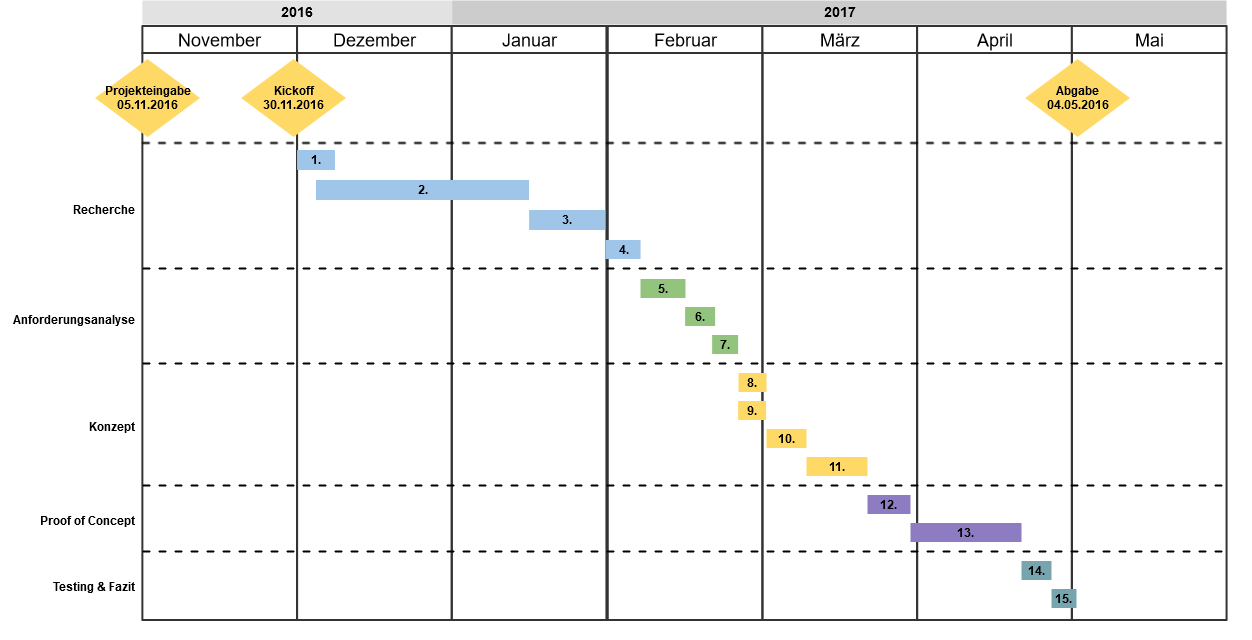
\includegraphics[width=1\textwidth]{images/projektablaufplan}
	\caption{Projektablaufplan}
	\label{fig:einleitung:projektablaufplan}
\end{sidewaysfigure}
\\\\
{\parindent0pt % disables indentation for all the text between { and }
Nachfolgend die Beschreibung der einzelnen Arbeitsschritte des Projektplanes.\\

Recherche:\\
1. Beschaffung der Buchungsdaten für die Auswertung.\\
2. Evaluation von verschiedenen Techniken des Data Mining, welche für die Auswertung der Daten verwendet werden können.\\
3. Vorhandene wissenschaftliche Arbeiten suchen, welche sich mit einer ähnlichen Problemstellung auseinandersetzen.\\
4. Evaluation von verschiedenen Programmen für die Auswertung und Darstellung der Daten.\\

Anforderungsanalyse:\\
5. Beschreibung der Vorgehensweisen, welche in wissenschaftlichen Arbeiten gefunden wurden und sich für die Problemstellung eignen. \\
6. Analyse der Buchungsdaten für die Auswertung.\\
7. Anforderungen an das Programm für die Auswertung und Darstellung der Daten.\\

Konzept:\\
8. Definition einer Vorgehensweise für die Datenanalyse.\\
9. Festlegen ob ein Programm für die Auswertung und Darstellung der Daten verwendet wird oder eine eigene Implementation.\\
10. Design und Funktionalität des Programmes definieren.\\
11. Definition der Testcases an das Programm.\\

Proof of Concept:\\
12. Vorbereitung der Daten für die Auswertung.\\
13. Erstellung oder Verwendung eines Programmes für die Analyse und Darstellung der Daten.\\

Testing \& Fazit\\
14. Auswertung der Testcases.\\
15. Einschätzung ob das Programm live für Interhome eingesetzt werden kann.
}

\section{Begriffsdefinition}
\label{sec:einletung:begriffsdefinition}
In der Arbeit werden durchgehend einige Begriffe verwendet welche hier erläutert werden. Für ein besseres Verständnis wird zuerst noch der Aufbau eines Objektes von Interhome aufgezeigt.

\cref{fig:einletung:begriffsdefinition:2} zeigt ein Objekt von Interhome wie es auf der Webseite \href{https://www.interhome.ch/de}{www.interhome.ch} gezeigt wird. Rot hinterlegt ist die Identifikation des Appartments. Diese wird ID oder im Interhome Jargon auch NREF genannt. Die grundlegenden Infos wie der Name des Objektes, wo es liegt, wie viele Sterne es hat, etc. ist im grünen Bereich ersichtlich. Die Preise und allfällige Aktionen sind im blauen Kasten und weitere Charakteristiken des Objektes zuunterst im gelben Bereich aufgeführt. Die Bilder werden in Analyse der Daten nicht verwendet weshalb sie nicht näher erläutert werden.
\begin{figure}[h]
	\centering
	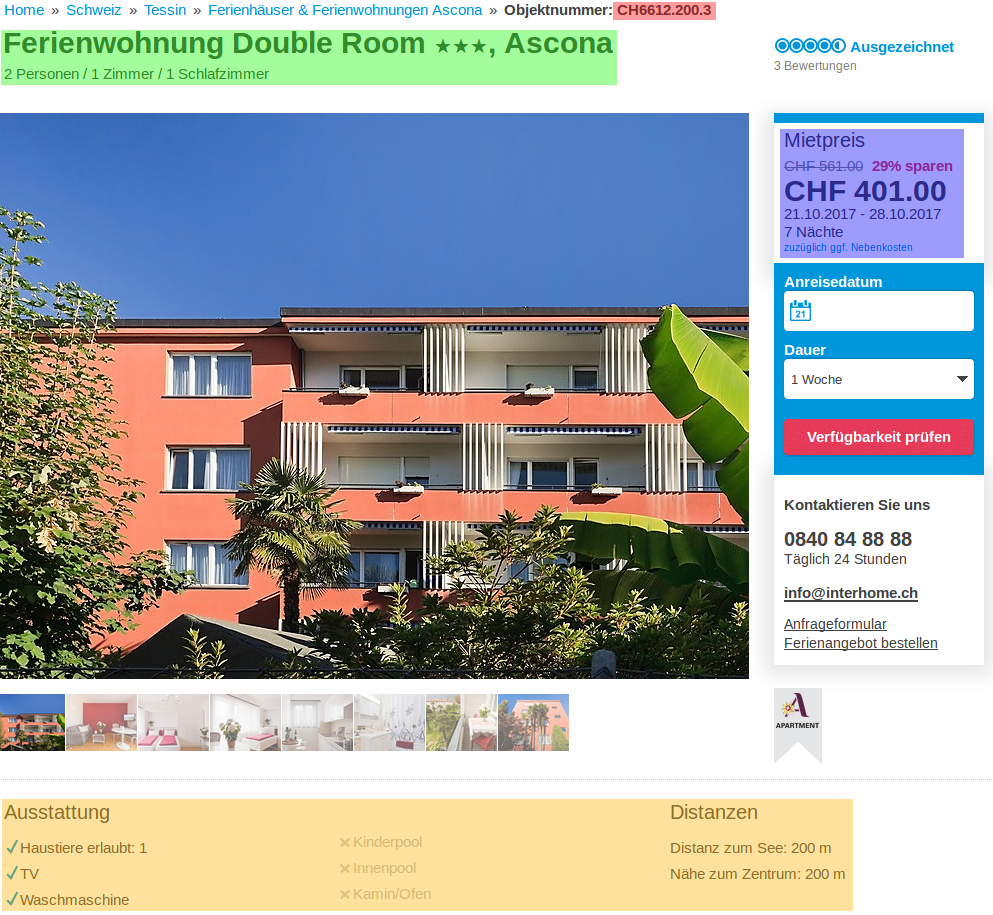
\includegraphics[width=1\textwidth]{images/interhome-object}
	\caption{Erklärung eines Interhome Objektes.}
	\label{fig:einletung:begriffsdefinition:2}
\end{figure}

Die zu erklärenden Begriffe sind in der \cref{fig:einletung:begriffsdefinition:1} aufgeführt. Diese werden im Text sowie in Formeln verwendet, weshalb zusätzlich zur Erklärung noch eine Variable definiert wurde.

\begin{table}[H] 
	\caption{Begriffsdefinition}
	\centering
	\rowcolors{1}{tablebodycolor}{tablerowcolor}
	\label{fig:einletung:begriffsdefinition:1}
	\begin{tabular}{ | c | C{2.5cm} | p{10cm} |} 
		\hline 
		\rowcolor{tableheadcolor}
		\bfseries Var & 
		\bfseries Begriff & 
		\bfseries Beschreibung \\ \hline 
		$A$ & Attribut & Ein Feld mit einem Wert. 1-n Attribute bilden eine Instanz. Beispiele:\
			\begin{itemize}
			\item ID: 5
			\item Distanz bis zum Meer: Nahe / Fern
			\item Sauna vorhanden: \checkmark
			\end{itemize} \\ \hline 
		$I$ & Instanz & Zusammenfassung von Attributen. 0-n Instanzen bilden eine Datenmenge. Nachfolgend wird ein Beispiel gezeigt, wie ein Objekt von Interhome vereinfacht aufgebaut sein könnte. Alle Attribute zusammen bilden eine Instanz.\
			\begin{itemize}
			\item ID: CH1000.400.1
			\item Preis (CHF): 500
			\item Sauna vorhanden: \checkmark
			\end{itemize} \\ \hline 
		$D$ & Datenmenge & In dieser Arbeit ist damit die Gesamtheit aller Buchungen von Interhome zu verstehen. Im folgenden Beispiel sind die Instanzen als Tupel dargestellt in der Form (ID, Preis, Anzahl Zimmer). Alle zusammen bilden die Datenmenge.\
			\begin{itemize}
			\item (CH1000.400.1, CHF500, 5)
			\item (CH1000.400.2, CHF340, 2)
			\end{itemize}\\ \hline 
		%$K$ & Konzept & Hypothesen über die Daten. \ z.B. Wenn jemand Bier kauft, dann meistens auch Windeln. \\ \hline 
		$A^c$ & Kategorische Attribute & Attribute welche eine endliche Anzahl von Ausprägungen annehmen können. In dieser Arbeit haben kategorische Attribute keine Reihenfolge. Z.B.: \
			\begin{itemize}
			\item Saune vorhanden: \checkmark, \ding{55}
			\item Distanz bis zum Meer: Nahe, Fern
			\end{itemize} \\ \hline
		$A^n$ & Numerische Attribute & Attribute welche eine reele Zahl $\mathbb{R}$ annehmen können.\\ \hline
		& i-Attributmenge & Eine Menge mit i Attributwerten. Z.B.:
			\begin{itemize}
			\item 1-Attributmenge: { (ID, 5) }
			\item 2-Attributmenge: { (ID, 5), (Preis, CHF500)}
			\end{itemize}\\ \hline 
	\end{tabular} 
\end{table}